% \iffalse
\let\negmedspace\undefined
\let\negthickspace\undefined
\documentclass[journal,12pt,twocolumn]{IEEEtran}
\usepackage{cite}
\usepackage{amsmath,amssymb,amsfonts,amsthm}
\usepackage{algorithmic}
\usepackage{graphicx}
\usepackage{textcomp}
\usepackage{xcolor}
\usepackage{txfonts}
\usepackage{listings}
\usepackage{enumitem}
\usepackage{mathtools}
\usepackage{gensymb}
\usepackage{comment}
\usepackage[breaklinks=true]{hyperref}
\usepackage{tkz-euclide} 
\usepackage{listings}
\usepackage{gvv}                                        
\def\inputGnumericTable{}                                 
\usepackage[latin1]{inputenc}                                
\usepackage{color}                                            
\usepackage{array}                                            
\usepackage{longtable}                                       
\usepackage{calc}                                             
\usepackage{multirow}                                         
\usepackage{hhline}                                           
\usepackage{ifthen}                                           
\usepackage{lscape}
\newtheorem{theorem}{Theorem}[section]
\newtheorem{problem}{Problem}
\newtheorem{proposition}{Proposition}[section]
\newtheorem{lemma}{Lemma}[section]
\newtheorem{corollary}[theorem]{Corollary}
\newtheorem{example}{Example}[section]
\newtheorem{definition}[problem]{Definition}
\newcommand{\BEQA}{\begin{eqnarray}}
\newcommand{\EEQA}{\end{eqnarray}}
\newcommand{\define}{\stackrel{\triangle}{=}}
\theoremstyle{remark}
\newtheorem{rem}{Remark}
\begin{document}

\bibliographystyle{IEEEtran}
\vspace{3cm}
\title{NCERT Question 11.9.3.9}
\author{EE23BTECH11019 - Faisal Imtiyaz $^{*}$% <-this % stops a space
}
\maketitle
\newpage
\bigskip

\renewcommand{\thefigure}{\arabic{figure}}
\renewcommand{\thetable}{\arabic{table}}


\vspace{3cm}
\textbf{Question:} Find the sum to indicated number of terms in the geometric progression:\\
$1,-a, a^2, -a^3,...n$ terms (if $a\neq-1$).\\
\solution
\begin{table}[htbp]
    \centering
    \def\arraystrech{1.5}
        \begin{tabular}{|p{2.5cm}|p{1.5cm}|p{3cm}|}
    \hline
            \textbf{Input Parameters} & \textbf{Values} & \textbf{Description} \\
    \hline
            $x(0)$ & $1$ & First term\\
    \hline
            $r$ & $(-a)$ & Common ratio\\
    \hline
            $x(n)$ & $(-a)^{n}u(n)$ & General term \\
    \hline
    \end{tabular}
    \caption{Given inputs}
    \label{tab:1.11.3.9}
\end{table} 
    
% \newline

\begin{table}[htbp]
    \centering
    \renewcommand{\arraystretch}{1.5}
    \begin{tabular}{|p{2.5cm}|p{3cm}|}
        \hline
        \textbf{Signal} & \textbf{Transform} \\
        \hline
        $\frac{1}{1-z^{-1}}$ & $u(n)$ \\
        \hline
        $\frac{1}{1-az^{-1}}$ & $(a)^{n}u(n)$ \\
        \hline
    \end{tabular}
    \caption{Z transform pairs}
    \label{pairs}
\end{table}
\begin{align}
x\brak{n} &= (-a)^{n}u(n)\\
X\brak{z} &=  \frac{1}{1+az^{-1}}
% \text{The ROC is :} \quad |z| > |a|\\
\end{align}
The ROC is $ \quad |z| > |a|$\\
% The ROC is:
% \begin{align}
%     \quad |z| > |a|\\
% \end{align}
% So essentially ROC is $ \quad |z| > \frac{1}{}$ > 1$\\
From \tabref{tab:1.11.3.9},
\begin{align}
% X\brak{z} =& \frac{1}{1+az^{-1}}\\
y\brak{n} &={(-a)^n}u(n)*u\brak{n}\\
Y\brak{z} &= X\brak{z}\ U\brak{z}\\
&=\frac{1}{1+az^{-1}}\frac{1}{1-z^{-1}}
\end{align}



Using Z transform pairs  to find the inverse Z-transform:\\
\begin{align}
    Y\brak{z}=& \frac{1}{a+1} \frac{1}{z^{-1}}\sbrak{\frac{1}{1-z^{-1}} - \frac{1}{1+az^{-1}}}\\
    y\brak{n} =&  \sbrak{\frac{1-(-a)^{n+1}}{1-(-a)}}u\brak{n}
\end{align}
\begin{figure}[ht!]
	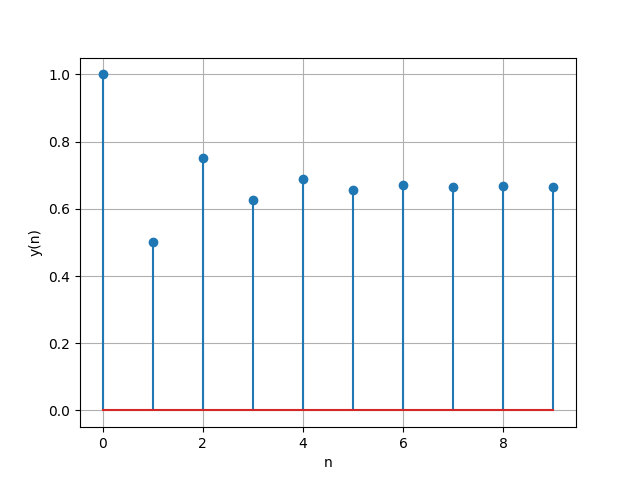
\includegraphics[width=\columnwidth]{plots/Figure_1.png}
	\caption{Plot of $y(n)$}
	\label{fig:1.2}
\end{figure}
\end{document}